\chapter*{Material Properties}
This appendix of material properties should be useful for initial comparison studies. For precise values several resources are recommend in a later section.


\begin{figure}[htbp]
  \centering
  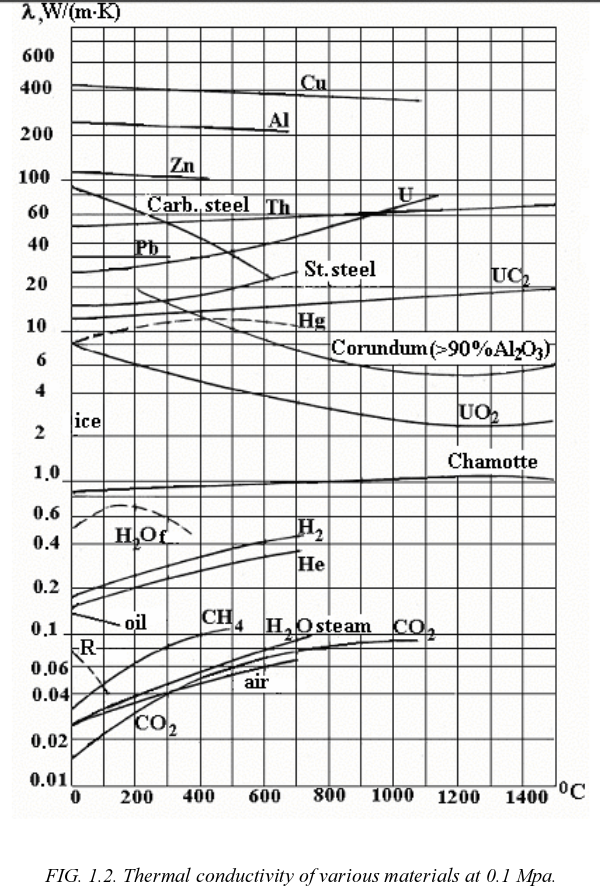
\includegraphics[width=4in]{graphics/thermal-k.png}  
  %\caption{Thermal conductivities}  
\end{figure}



\begin{table}
  \centering
  \caption{Basic Thermal Properties\cite{IAEA_1}}
  \begin{tabular}{lcccc}
    \toprule  
    Material & Conductivity & Density & Melting Point & Thermal Expansion\\ 
    %Heat Capacity,K/W/g
             & W/mK &    g/cm$^3$     &   $^{\circ}$C  &  1E6/$^{\circ}$C \\
    \midrule    
    UO$_2$ & 2.79 & 10.963 & 2800 & 9.8\\
    UN     & 20.9 & 14.42  & 2850 & 7.5\\
    UC     & 23   & 13.63  & 2365 & 10.5\\
    U metal & 31.2 & 19.1  & 1130 & 13.9\\
    U-20Pu-10Zr & 16 & 15.67 & 1155 &17\\
    U$_3$Si$_2$ & 22 & 12.2  & 1700 &16.1 \\
    \bottomrule
  \end{tabular}

\end{table}


A good resource has been provided by the IAEA\cite{IAEA_1}.


%%%%%%%%%%%%%%%%%%%%%%%%%%%%%%



\bibliographystyle{ieeetr}
\bibliography{matbib}


